% Flavor anomalies (LHCb)

The SM assumes that the weak gauge bosons couple to each lepton flavor identically (or close to it), a phenomenon called lepton flavor universality. Tests of lepton flavor universality can be performed by studying flavor-changing neutral current (FCNC) transitions, such as when a bottom quark transforms into strange quark in the decay: \HepProcess{\PB \to \PK\Pleptonplus\Pleptonminus}. As FCNC are suppressed at tree-level in the SM, occuring only via higher order electroweak processes (as shown in the left-hand diagram of Fig.~\ref{fig:FCNC}), these decays are a powerful probe into new physics. Measurements by the LHCb, BaBar, and Belle collaborations of observables such as \Ratio{\PK}, \Ratio{\PKstar}, \Ratio{\PD}, and \Ratio{\PDstar}---the decay branching fractions of \PB mesons into an electron-positron pair over a muon-antimuon pair---hint at a possible violation of lepton flavor universality. Combining the flavor anomalies from each collaboration in \Ratio{\PKstar} (Fig.~\ref{fig:FlavorAnomalies}, left) yields tension between experiment and the SM at 2 standard deviations~\cite{LHCb1}, and for \Ratio{\PK} (Fig.~\ref{fig:FlavorAnomalies}, right) up to 3.1 standard deviations~\cite{LHCb2}. Leptoquarks coupling to muons and bottom quarks are prime candidates to explain these flavor anomalies at tree-level, as shown in the right-hand diagram of Fig.~\ref{fig:FCNC}.

\begin{figure}[H]
    \centering
    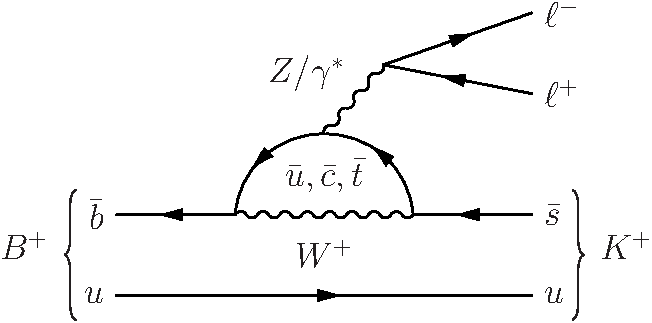
\includegraphics[width=0.4\textwidth]{Images/Theory/BplusDecayFCNC.pdf}\hspace{0.1\textwidth}
    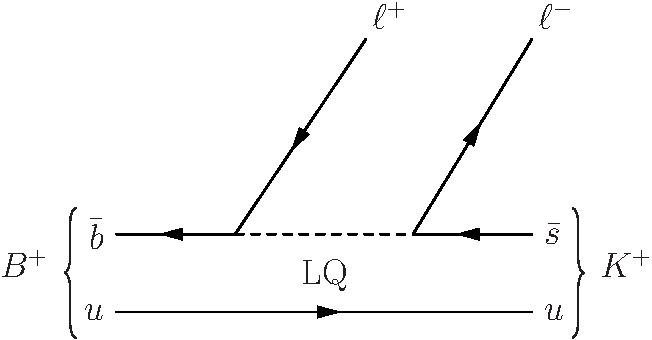
\includegraphics[width=0.4\textwidth]{Images/Theory/BplusDecayLQ.pdf}
    \caption{The decay of a charged \PB meson into a charged kaon and a pair of opposite-sign charged leptons. Left: An example of a loop diagram FCNC process in the SM that is strongly suppressed. Right: A tree-level FCNC solution with a leptoquark mediating the transition.}
    \label{fig:FCNC}
\end{figure}

\begin{figure}[H]
    \centering
    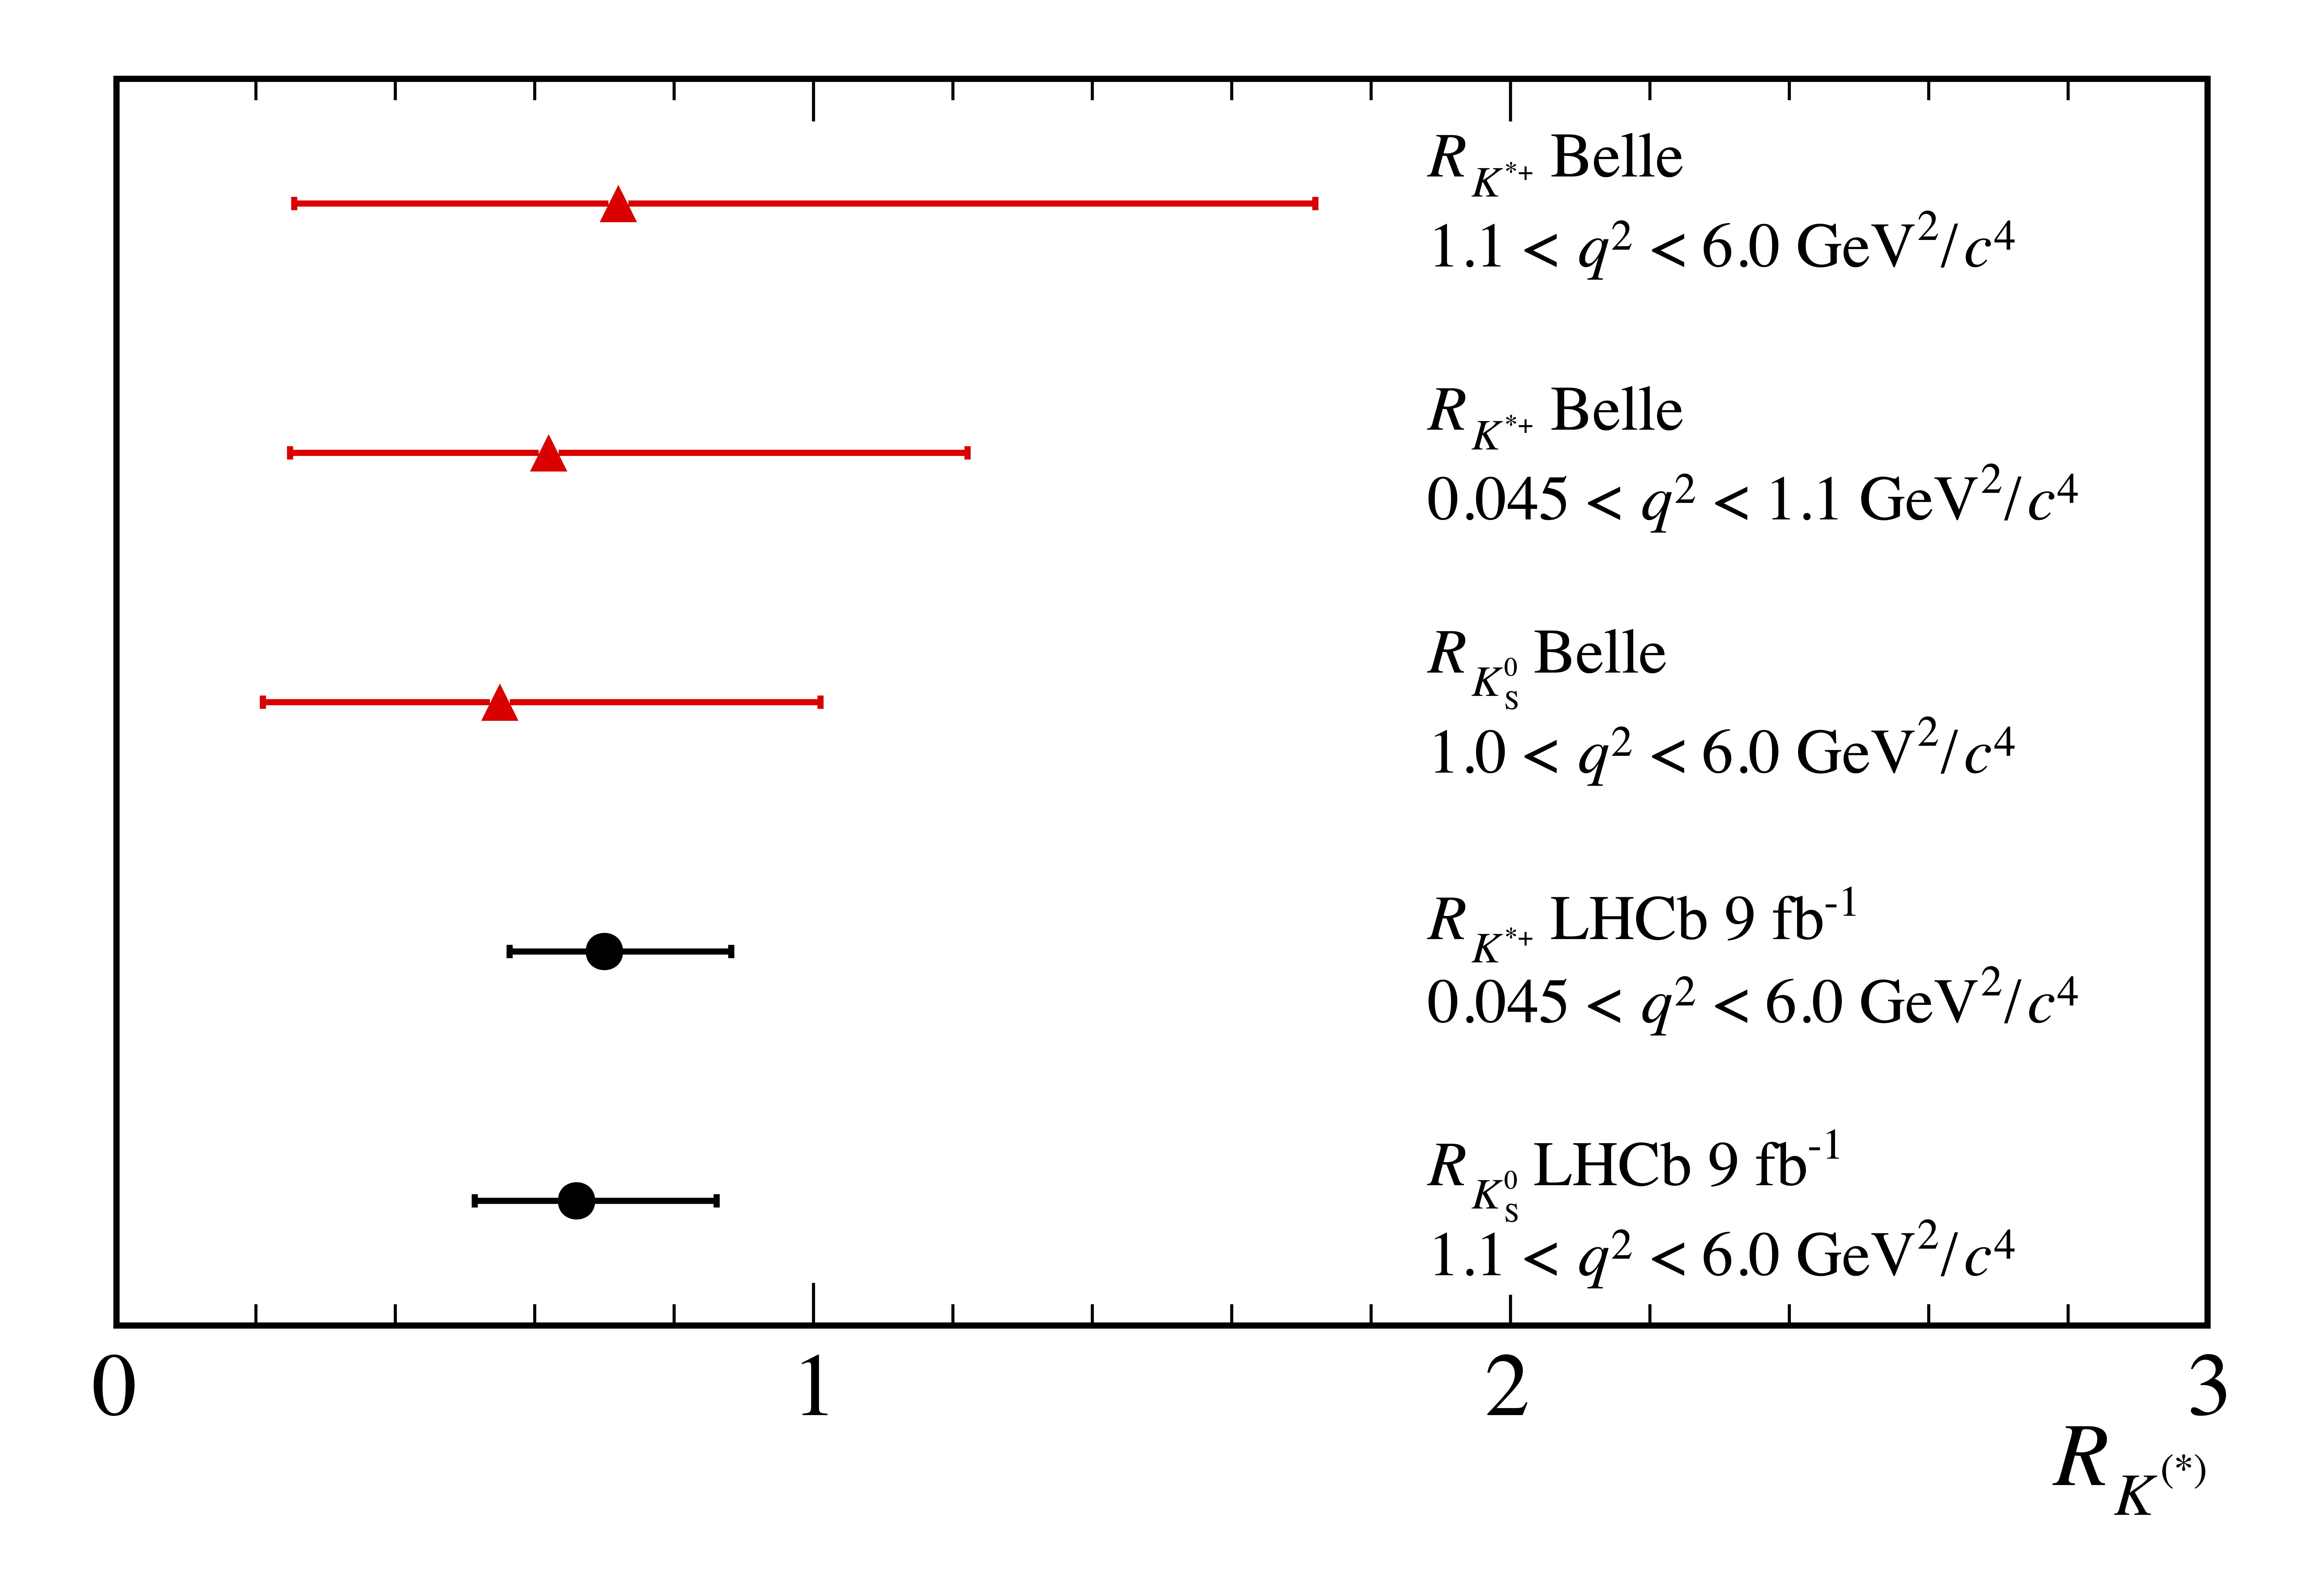
\includegraphics[width=0.49\textwidth]{Images/Theory/LHCbBelle.png}
    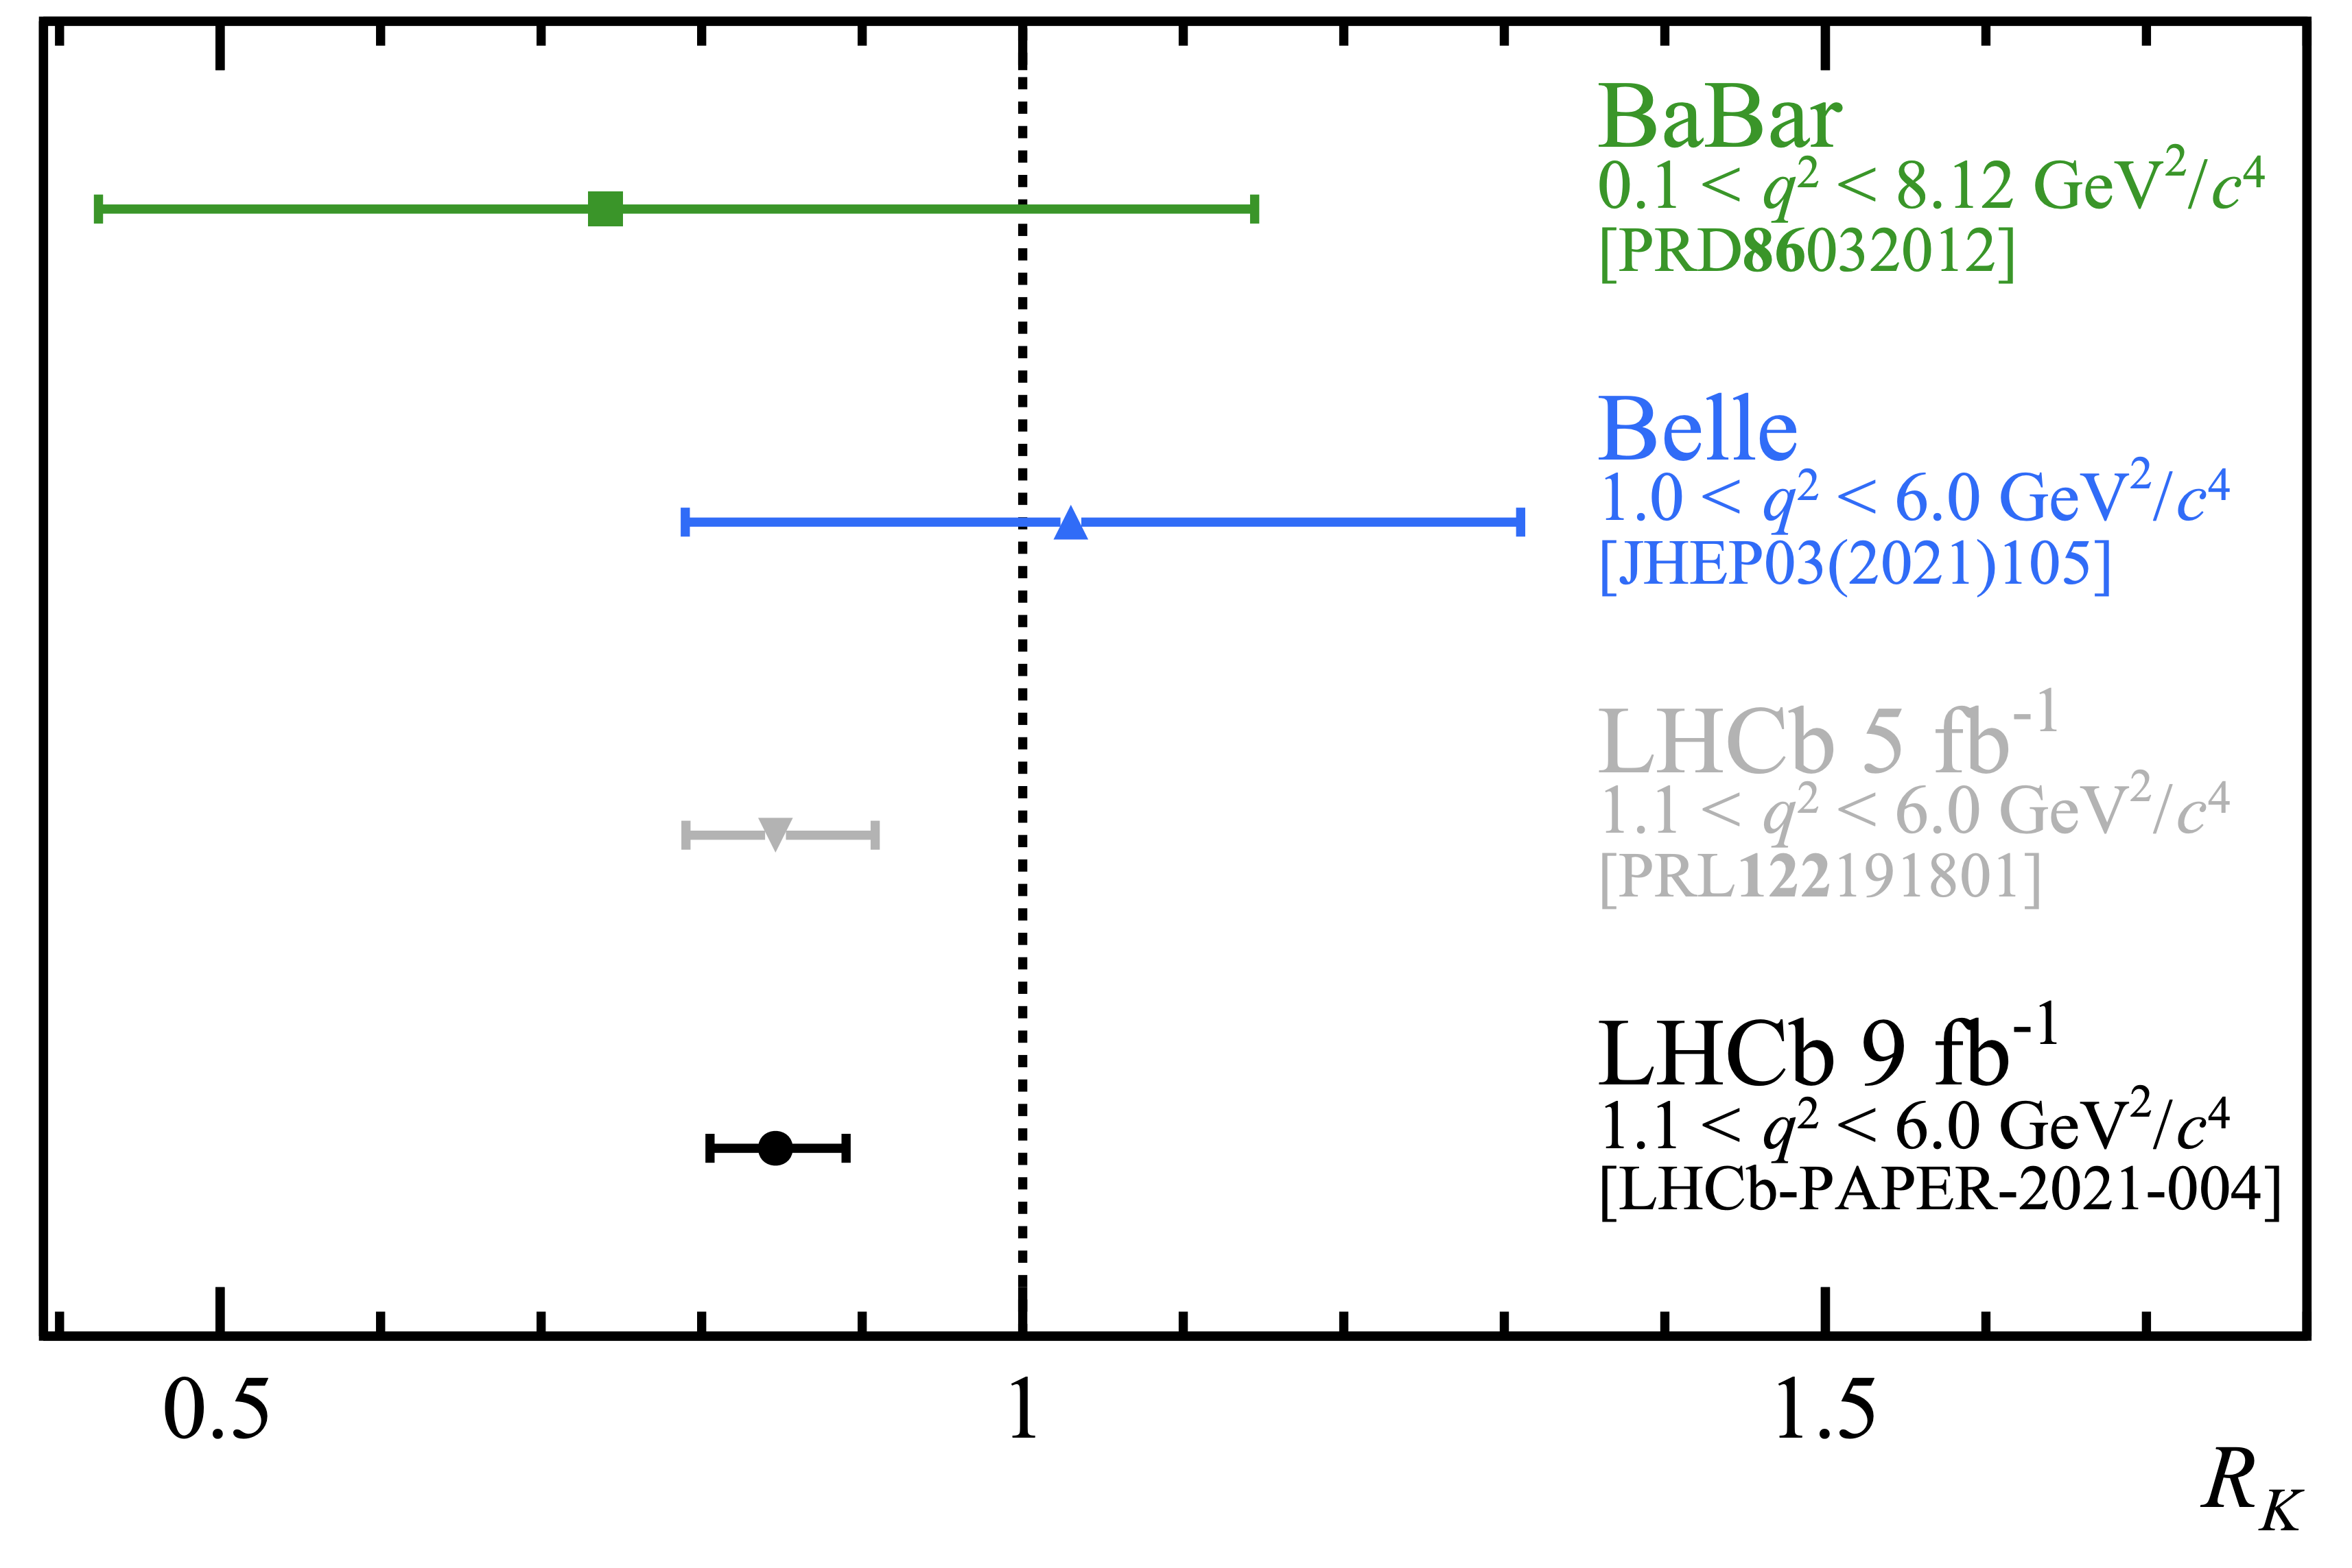
\includegraphics[width=0.49\textwidth]{Images/Theory/RKmeasurements.png}
    \caption{Left: A comparison of \Ratio{\PKstar} measurements by the Belle and LHCb collaborations for several bands of the dilepton invariant mass squared $q^2$. Right: A comparison of \Ratio{\PK} measurements (combining \HepProcess{\PBplus \to \PKplus\Pleptonplus\Pleptonminus} and \HepProcess{\PBzero \to \PKzero\Pleptonplus\Pleptonminus} decays) by the BaBar, Belle, and LHCb collaborations for several bands of the dilepton invariant mass squared $q^2$.}
    \label{fig:FlavorAnomalies}
\end{figure}

% Muon magnetic moment anomaly (Muon g-2)

Another notable inconsistency between the SM prediction and experiment in which leptoquarks may play a role is the anomalous muon magentic dipole moment. The magnetic moment of the muon is defined as:

\begin{equation}
    \vec{\mu} = \gmuon\left(\frac{q}{2m_{\Pmu}}\right)\vec{s}
\end{equation}
where the factor \gmuon as predicted by the Dirac equation is equal to 2. Considering a number of EM, EW, and QCD radiative corrections (a few example diagrams are shown in Fig.~\ref{fig:amu}, left), the SM value of \gmuon is predicted with high precision to deviate from 2, encapsulated in the muon magnetic anomaly $\amuon = (\gmuon-2)/2$. Recent calculations set the SM theoretical value $\amuon(\mathrm{SM})=\num{116591810(43)e-11}$, a precision of 0.37 parts-per-million (ppm). Measurements of \amuon by the Muon $g-2$ experiment at Brookhaven National Laboratory (BNL) and Fermilab National Accelerator Laboratory (FNAL) found a combined experimental average of $\amuon(\mathrm{Exp}) = \num{116592061(41)e-11}$, with an astonishing precision of 0.34 ppm~\cite{Muongminus2}, as shown in Fig.~\ref{fig:amuExp}. The difference between the theoretical prediction and the experimental average has a significance of 4.2 standard deviations. Introducing leptoquarks that couple to muons could explain the deviation form the SM, as seen in the diagram in Fig.~\ref{fig:amuLQ}.

\begin{figure}[H]
    \centering
    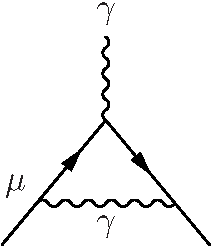
\includegraphics[width=0.2\textwidth]{Images/Theory/Muon_gminus2_photon.pdf}\hspace{0.05\textwidth}
    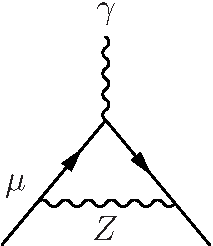
\includegraphics[width=0.2\textwidth]{Images/Theory/Muon_gminus2_Z.pdf}\hspace{0.05\textwidth}
    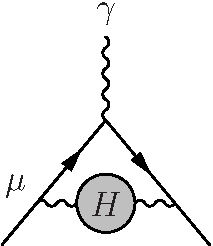
\includegraphics[width=0.2\textwidth]{Images/Theory/Muon_gminus2_Hadronic.pdf}\hspace{0.05\textwidth}
    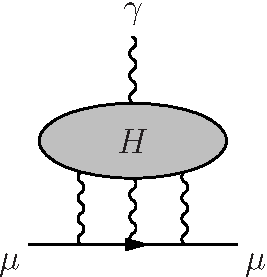
\includegraphics[width=0.2\textwidth]{Images/Theory/Muon_gminus2_Hadronic2.pdf}
    \caption{The Feynman diagrams of SM contributions to the muon anomaly. From left to right: the first-order QED and weak processes, leading-order hadronic vacuum polarization, and hadronic light-by-light contributions.}
    \label{fig:amu}
\end{figure}

\begin{figure}[H]
    \centering
    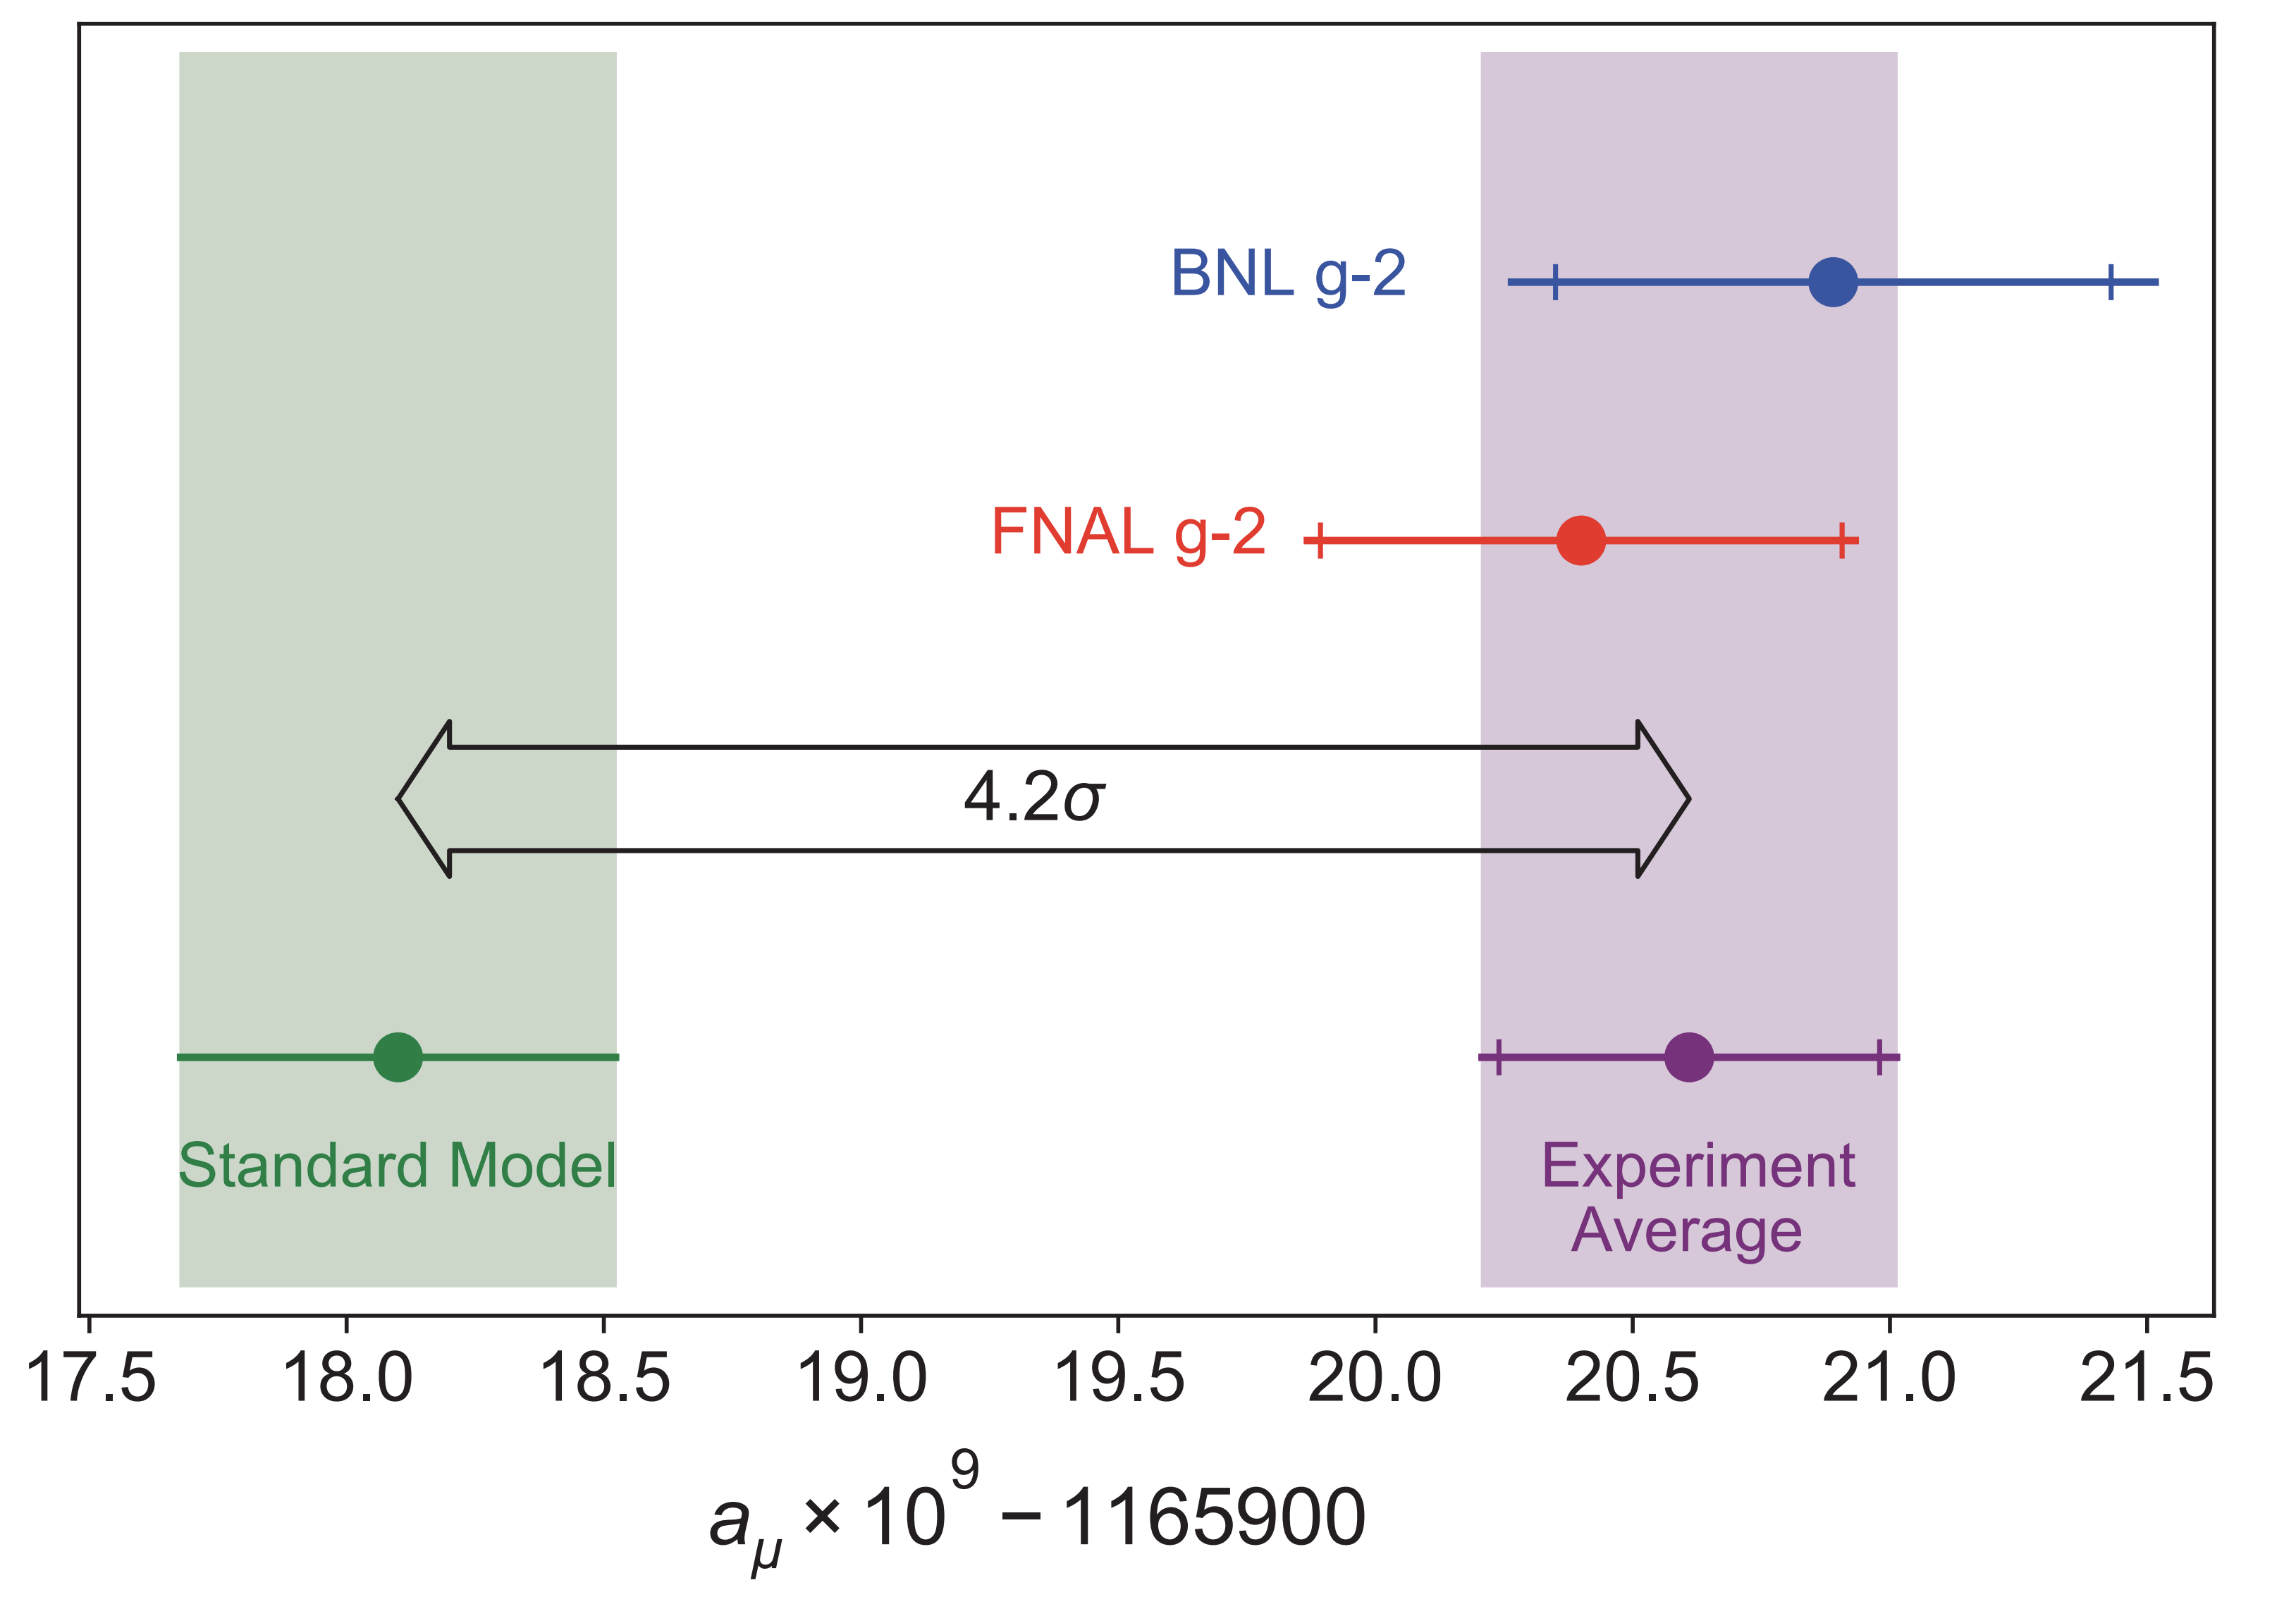
\includegraphics[width=0.7\textwidth]{Images/Theory/MuonAnomaly.png}
    \caption{A comparison of \amuon measured by BNL, FNAL, and the combined average beside the SM prediction.}
    \label{fig:amuExp}
\end{figure}

\begin{figure}[H]
    \centering
    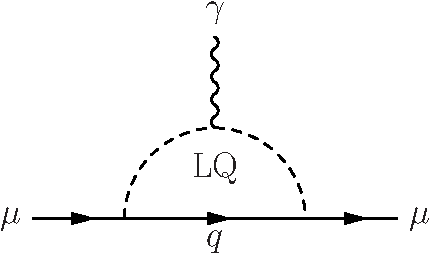
\includegraphics[width=0.5\textwidth]{Images/Theory/Muon_gminus2_LQ.pdf}
    \caption{A Feynman diagram of a leptoquark solution to the magnetic anomaly \amuon.}
    \label{fig:amuLQ}
\end{figure}